\newpage
\section{System Specifications and Technological Stack}
This section of the elaborate will involve the discussion of the system requirements, as well as how the system have been designed. Finally, the technological stack and the major tools adopted for the project will be covered, such as the programming languages, IDE, libraries, automation dependency tools.
\subsection{System Requirements}
Given the fact that this project was already existing, it had some implemented features (and consequently some basic requirements related to them), our work was based on extending the app capabilities by implementing new features or refactor existing ones. \newline Considering this aspect, I will classify the functional requirements that regards our work as follows:
% 
% ROSSI DA RIVEDERE, SE FACCIAMO ANCHE LE LEZIONI AGGIUNGERE ANCHE QUELLE
%     
\begin{table}[h!]
    \centering
    \begin{tabular}{|>{\raggedright\arraybackslash}p{0.1\linewidth}|>{\raggedright\arraybackslash}p{0.2\linewidth}|>{\raggedright\arraybackslash}p{0.6\linewidth}|}
        \hline
        \textbf{FR1} & \multicolumn{2}{>{\centering\arraybackslash}p{0.7\linewidth}|}{\textbf{User Management}} \\
        \hline
        FR 1.1 & Home Page & Allow a user to enter and also visualize data regarding his emotional state. \\
        \hline
        FR 1.2 & Home Page & Allow a user to visualize data on the charts that exceeds the related goals differently (they visually differ from the other ones). \\
        \hline
        FR 1.3 & Health Measures Page & Allow a user to view his vital metrics by using charts organized in different tabs instead of raw values, for a better understanding. \\
        \hline
        FR 1.4 & Personal Information Page & Allow a user to provide his personal measures as well as his activity goals, used as upper bound into the charts of the Home Page. \\
        \hline
        FR 1.5 & Notification System & Allow a user to receive notification with different frequencies to prompt him into inserting data regarding food, emotional aspect, balance capability, strenght capability. \\
        \hline
        FR 1.6 & \textcolor{red}{Assessment} & Allow a user to visualize a periodic assessment produced thanks to the data that were previously inserted. \\
        \hline
        FR 1.7 & \textcolor{red}{User Registration} & Allow a user to enter his demographics (age,sex,...) and body (height,weight,...) data when the registration is in progress. \\
        \hline
    \end{tabular}
    \caption{Overview of Functional Requirements related to the User Management.}
\end{table}

\newpage

\begin{table}[h!]
    \centering
    \begin{tabular}{|>{\raggedright\arraybackslash}p{0.1\linewidth}|>{\raggedright\arraybackslash}p{0.2\linewidth}|>{\raggedright\arraybackslash}p{0.6\linewidth}|}
        \hline
        \textbf{FR2} & \multicolumn{2}{>{\centering\arraybackslash}p{0.7\linewidth}|}{\textbf{Data Management}} \\
        \hline
        FR 2.1 & Data Source Migration & Migrating the main app data source from FitBit Server to Health Connect and Apple Health (Health data management and integration platforms, developed by Google and Apple respectively), while still keeping Google Firebase as additional data source. \\
        \hline
        FR 2.2 & User Goal Data Integration & Allow a user to retrieve, visualize, insert and edit his goals. \\
        \hline
        FR 2.3 & User Emotional Data Integration & Allow a user to retrieve, visualize and insert his emotional data, based on the selected time period. \\
        \hline
        FR 2.4 & Health Data Backup & Added the necessary logic to perform a backup of the users's health data. \\
        \hline
        FR 2.5 & \textcolor{red}{Food Data Integration} & Allow a user to insert his food data once received the notification. \\
        \hline
        FR 2.6 & \textcolor{red}{Emotional Data Integration} & Allow a user to insert his emotional data once received the notification. \\
        \hline
        FR 2.7 & \textcolor{red}{Balance Capability Data Integration} & Allow a user to insert his balance capability data once received the notification. \\
        \hline
        FR 2.8 & \textcolor{red}{Strenght Capability Data Integration} & Allow a user to insert his strength capability data once received the notification. \\
        \hline
    \end{tabular}
    \caption{Overview of Functional Requirements related to the Data Management.}
    \label{tab:fr2}
\end{table}

\clearpage

\noindent As far as concerns the non-functional requirements, we can classify them as follows:

\begin{table}[h!]
    \centering
    \begin{tabular}{|>{\raggedright\arraybackslash}p{0.1\linewidth}|>{\raggedright\arraybackslash}p{0.2\linewidth}|>{\raggedright\arraybackslash}p{0.6\linewidth}|}
        \hline
        \textbf{NFR} & \textbf{Type} & \textbf{Description} \\
        \hline
        NFR1 & Reliability & The system should ensure at least 80\% accuracy and functionality over the course of a year. \\
        \hline
        NFR2 & Portability & The application must be capable of running on Android and IOS devices. \\
        \hline
        NFR3 & Security & Robust login mechanisms should be implemented to protect user data and limit access only to authorized individuals. \\
        \hline
        NFR4 & Usability & The application should be intuitive enough for users of all ages and skill levels, requiring minimal training. \\
        \hline
        NFR5 & Data Privacy & User data must adhere to OAUTH for secure data handling. \\
        \hline
        NFR6 & Performance & The app should smoothly load and handle user interactions within two seconds under typical conditions in order to achieve an optimal user experience. \\
        \hline
        NFR7 & Interoperability & The application should seamlessly connect with third-party platforms like Health Connect and Apple Health, maintaining data accuracy and improving functionality. \\
        \hline
        NFR8 & Localization & The app should support at least English and Italian languages, adapting content and formats (e.g., date, currency) accordingly. \\
        \hline
        NFR9 & Modularity & The app's architecture should support modular development to facilitate future updates without impacting the entire codebase. \\
        \hline
    \end{tabular}
    \caption{Overview of Non-Functional Requirements related to the system.}
\end{table}
\newpage
\subsection{System Architecture And Design}
Focusing on the system architecture and his design, it can be summarized as follows:
\begin{figure*}
    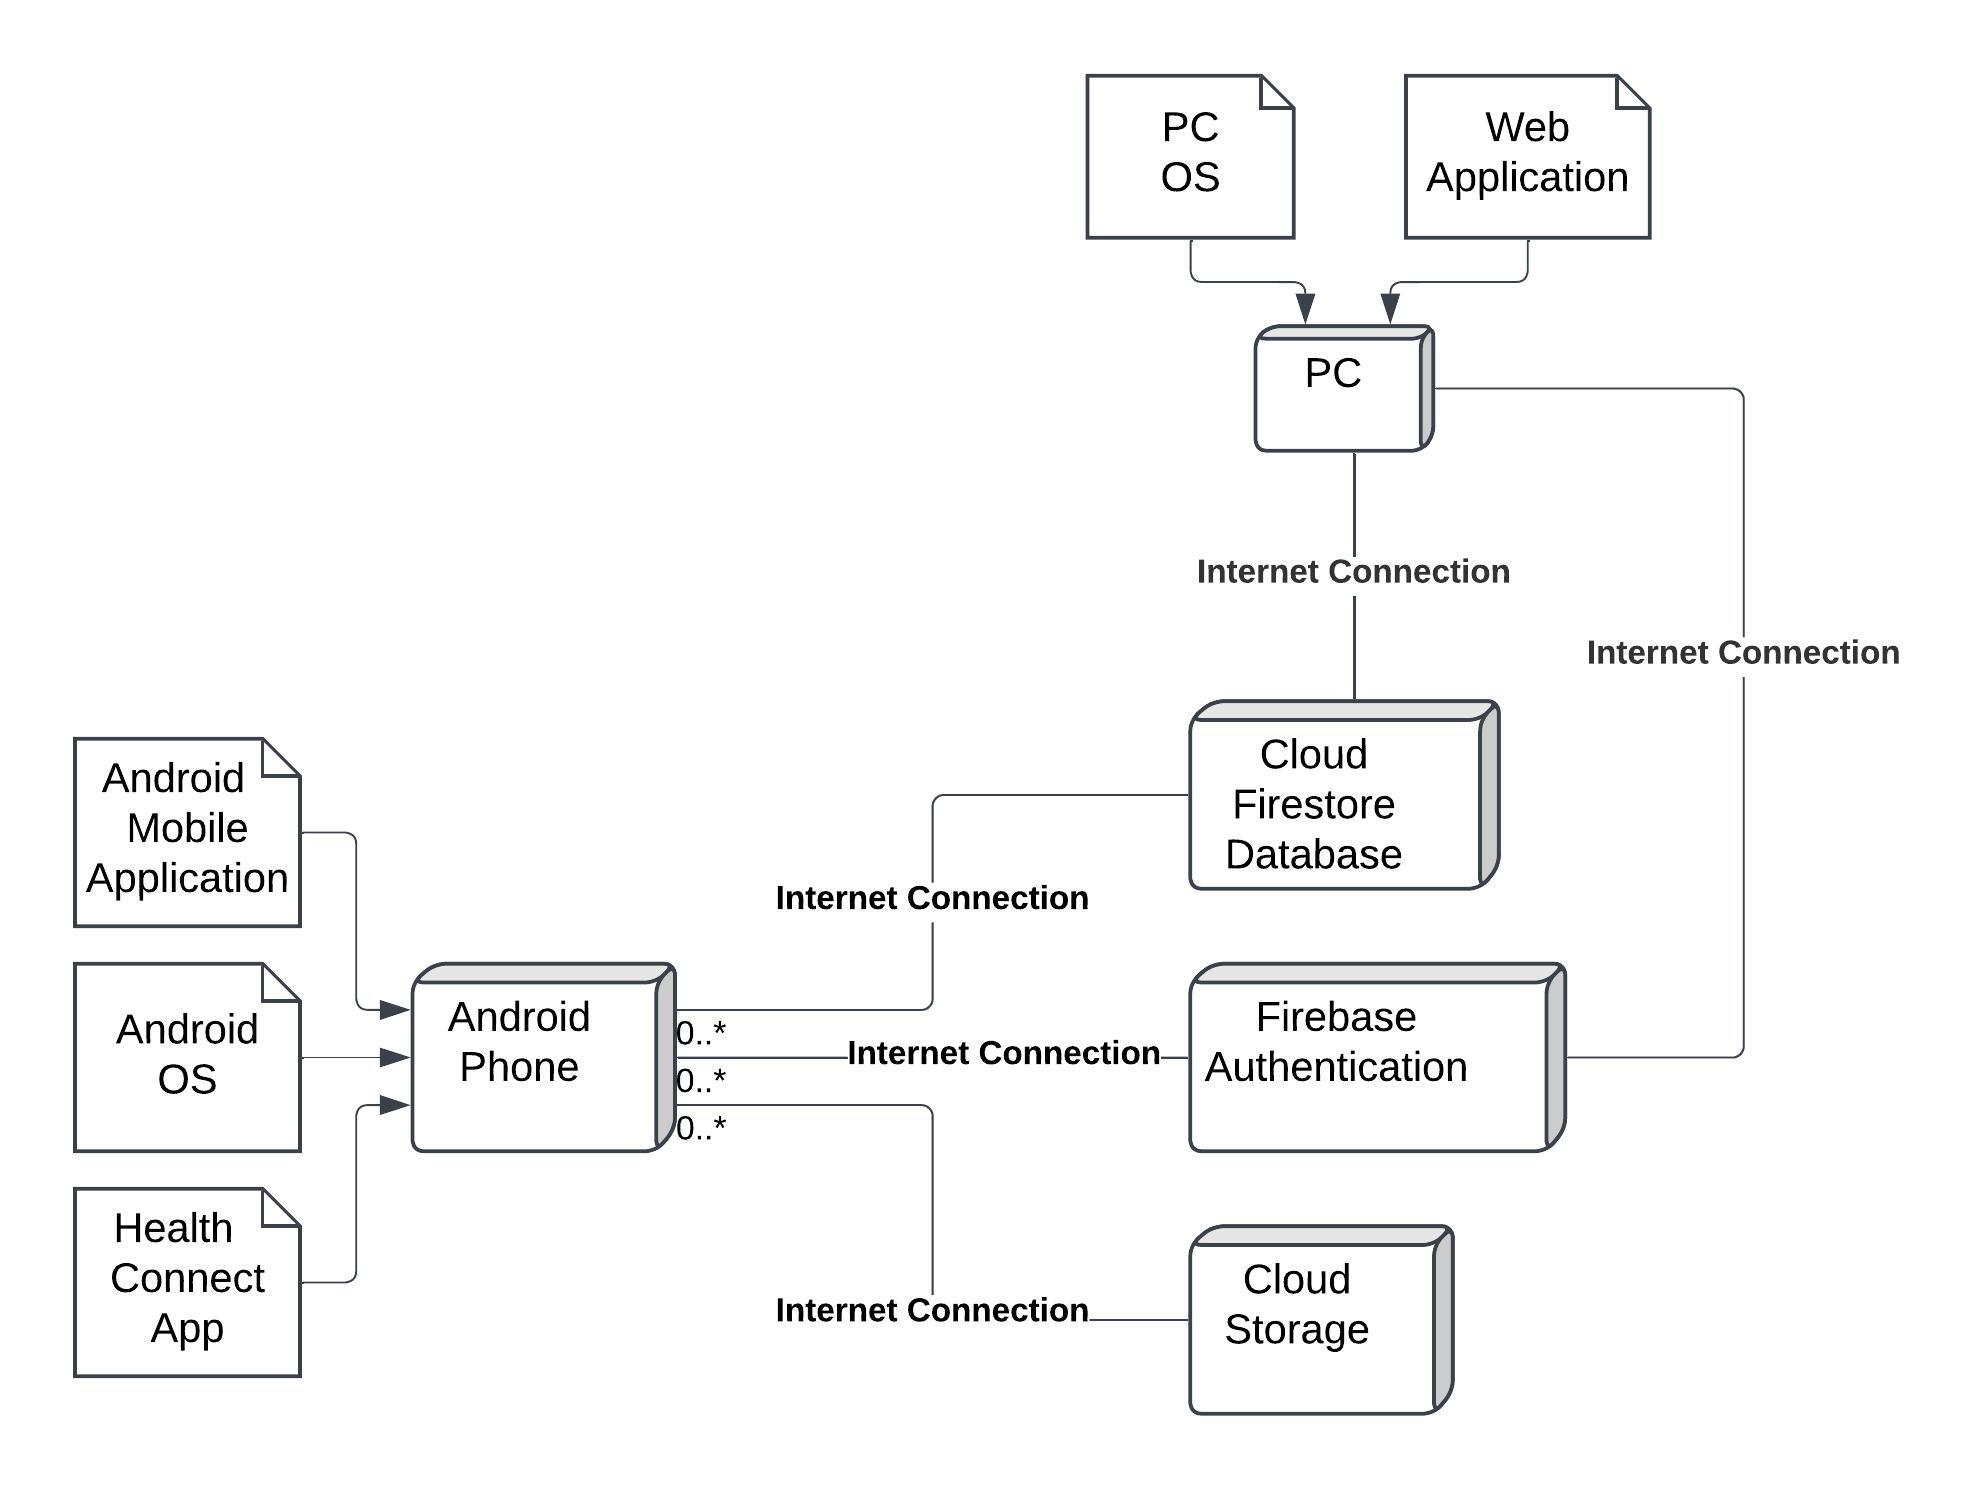
\includegraphics[width=1.0\linewidth]{./images/system_architecture.jpeg}
    \caption{Overview of the System Architecture.}
    \label{fig:systemArchitecture}
\end{figure*}

\noindent We can clearly distinguish the two main use cases (Android and IOS) with their distinguishing components and the common ones:

\begin{itemize}[nosep] % 'nosep' removes extra spacing between items
    \item Android Architecture:\vspace{2ex}
          \begin{itemize}[nosep]
              \item \textbf{Android Phone} that represent the physical smartphone, along with his operating system, our application installed and health connect installed, used to manage the health data on Android, that further interacts with google fit server whenever is needed.
              \item \textbf{Google Fit} server, used among the health connect app data sources.
              % Questo eprchè nei settings di health connect si può scegliere se usare google fit e altre sorgenti anche la nostra app c'è
          \end{itemize}
          \vspace{3ex}
    \item IOS Architecture:\vspace{2ex}
          \begin{itemize}[nosep]
              \item \textbf{Apple IPhone} that represent the physical smartphone, along with his operating system, our application installed and apple health installed, used to manage the health data on IOS, that interacts with apple health server whenever is needed.
              \item \textbf{Apple Health} server, used as data source for the apple health application.
          \end{itemize}
          \vspace{10ex}
    \item Common Components:\vspace{2ex}
          \begin{itemize}[nosep]
              \item \textbf{Firebase Authentication Service} server, employed in order to perform and enforce authentication.
              \item \textbf{Google Firebase} employed as a data source for the application logic, containing other needed data, such as profile information, in addition to the backup of the health data for each user (see \cref{tab:fr2} FR 2.1) stored in Firebase Storage, Google Firebase service focused on storing user-generated content such as photos, videos, and other types of files.
              \item A \textbf{Large Language Model} pre-trained and then fine tuned on the health data of the users employed to generate recommendation for the user. 
              \item A \textbf{Personal Computer} along with his operating system and a web application that allows to interact with the llm on administrator side \textcolor{red}{to adjust recommendation as well as editing sentences that prompt the user into inserting data.}  
          \end{itemize}
\end{itemize}
\vspace{3ex}

\noindent In addition to this architecture, the system can be further enriched by integrating a wearable device, that can be a very useful tool to gather data, as previously explained in \cref{sec:wearableDevices}. In this scenario the wearable device will be connected to the smartphone:

\begin{figure*}
    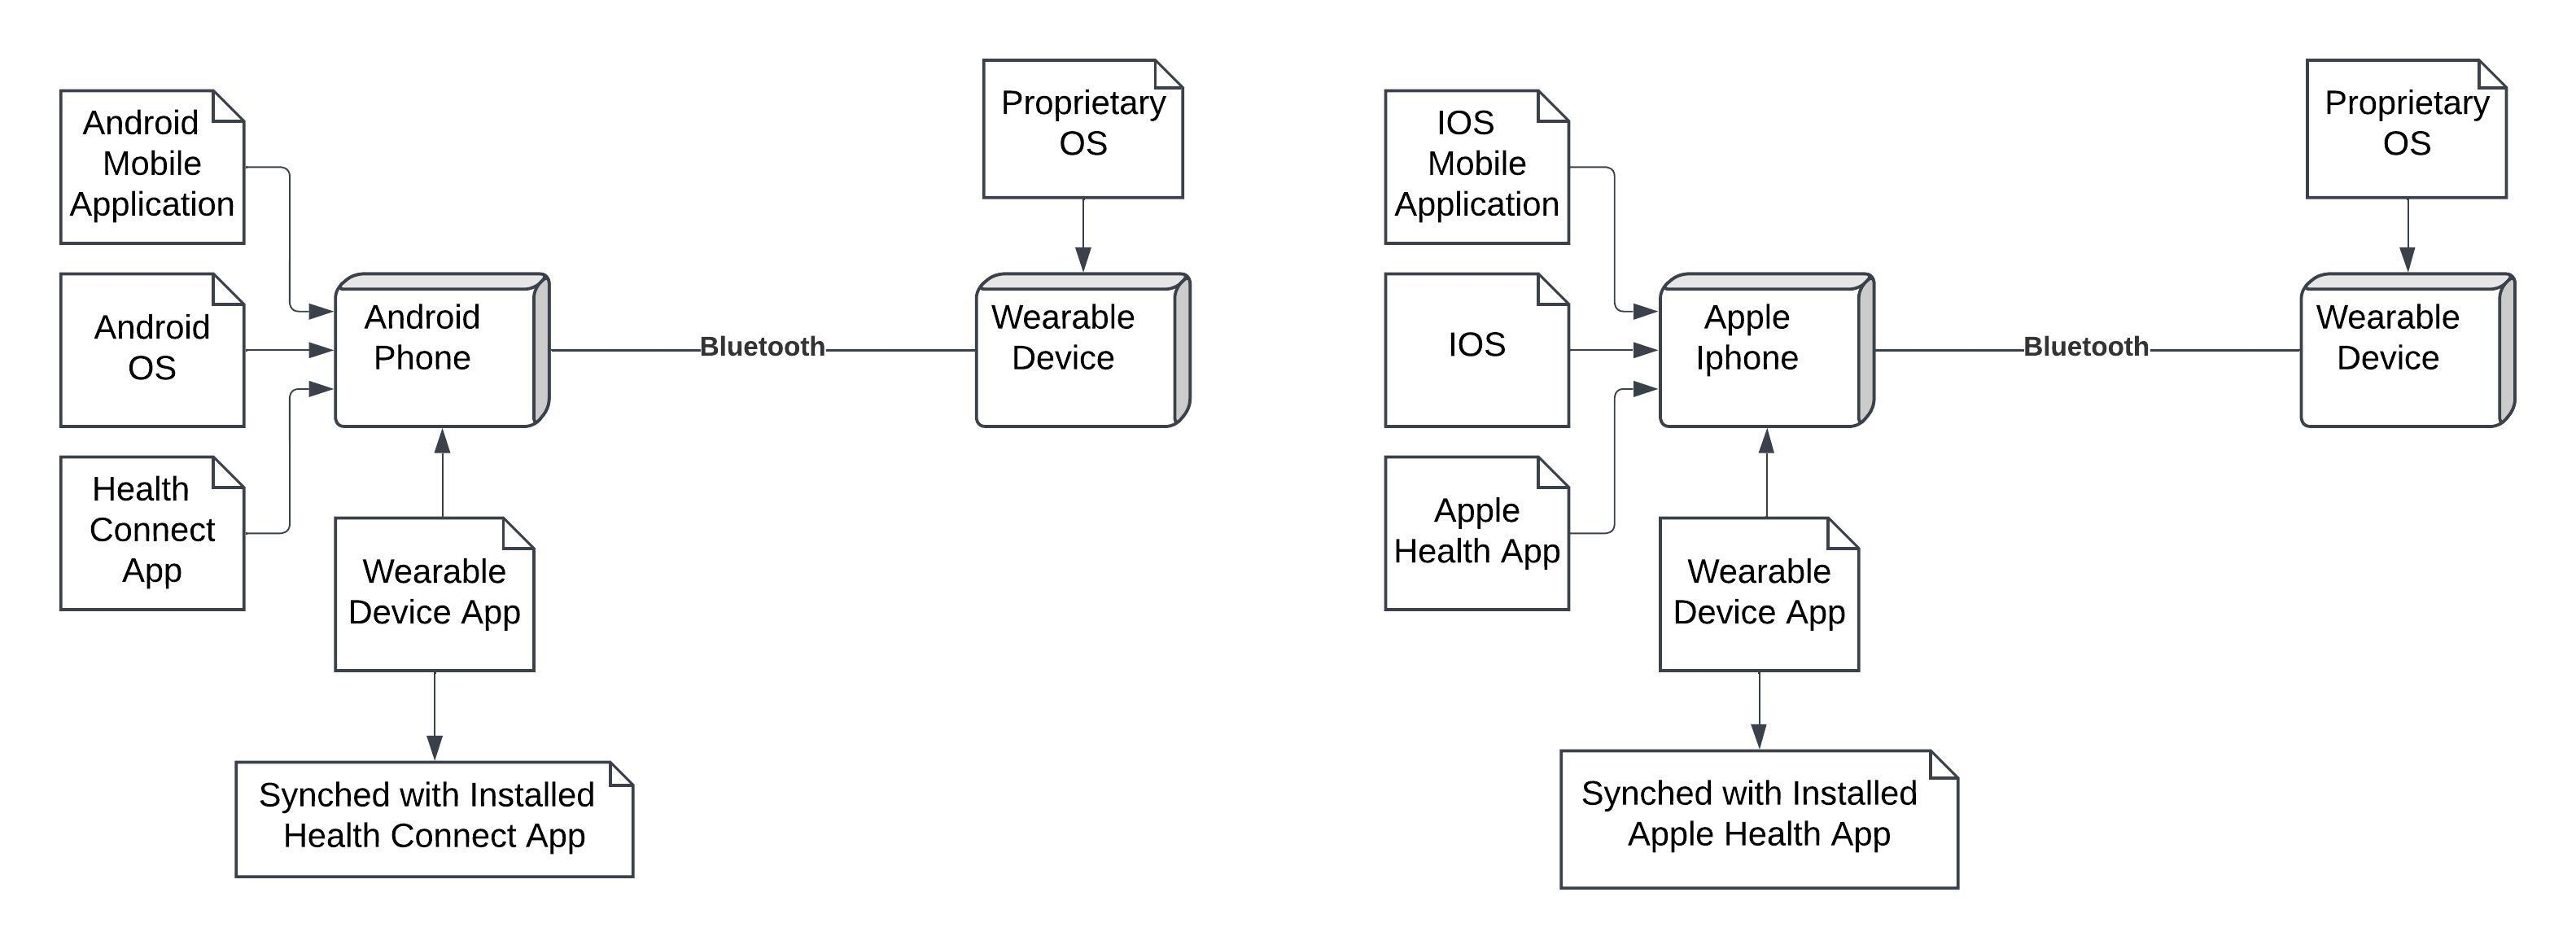
\includegraphics[width=1.0\linewidth]{./images/system_architecture_wearable.jpeg}
    \caption{Overview of the Mobile System Architecture with Wearables.}
    \label{fig:systemArchitectureWearables}
\end{figure*}

\noindent In this case the architecture has been extended with the wearable devices, along with his operating system, that throuugh bluetooth connection can communicate with the smartphone (Android or IOS). On the smartphone side, the wearable application will be able to retrieve the data from the wearable device to then sync with the respective data management service (respectively Health Connect or Apple Health).

\subsection{Technological Stack}